\documentclass[10pt]{article}
\usepackage[paperwidth=105mm,paperheight=148mm,hmargin=1cm,top=1cm,bottom=1.75cm]{geometry}
\usepackage{fontspec}
\usepackage[PunctStyle=plain]{xeCJK}
\usepackage[shortlabels,inline]{enumitem}
\usepackage{amsmath}
\usepackage{amssymb}
\usepackage{caption}
\usepackage{chemformula}
\usepackage{siunitx}
\usepackage{tikz}
\usepackage{xeCJKfntef}
\usepackage{pgfplots}
\usepackage{lastpage}
\usepackage{fancyhdr}
\usepackage{needspace}

\pretolerance=5000
\tolerance=9000
\emergencystretch=10pt

\pagestyle{fancy}
\renewcommand{\headrulewidth}{0pt}
\fancyhead{}
\cfoot{\footnotesize\thepage\ /\ \pageref{LastPage}}
\setlength{\parindent}{0pt}
\setCJKmainfont[BoldFont=Noto Serif CJK TC SemiBold]{Noto Serif CJK TC}
\linespread{1.15}

\usepackage{tabto}
\newenvironment{choice}{\begin{enumerate}[label=(\Alph*),align=left,leftmargin=*,labelsep=.3em,topsep=0ex,itemsep=0ex]}{\end{enumerate}}
%\newenvironment{choices}[1]{\par\NumTabs{#1}\begin{enumerate*}[label=(\Alph*),itemjoin=\tab]}{\end{enumerate*}}

\newcommand*{\blank}[1]{\rule[-.7\baselineskip]{0pt}{1.8\baselineskip}\fbox{\rule[-.4\baselineskip]{0pt}{1.2\baselineskip}\hspace{#1}}}
\newcommand*{\fraction}[2]{\rule[-.8\baselineskip]{0pt}{2\baselineskip}\dfrac{#1}{#2}}
\newcommand*{\sfraction}[2]{\rule[-.4\baselineskip]{0pt}{1.2\baselineskip}\tfrac{#1}{#2}}

\usepackage{titlesec}
\usepackage{zhnumber}
\titleformat{\section}{\normalfont\bfseries}{{\thesection}、}{0em}{}
\titlespacing{\section}{0pt}{2ex plus .5ex minus .2ex}{1.3ex plus .2ex}
\renewcommand{\thesection}{\zhnum{section}}

\makeatletter
\renewcommand*{\maketitle}{{%
  \bfseries
  \LARGE 練習(數學) \\
  \large 多項式的除法、一次與二次函數、三次函數 \par
}}
\makeatother

\begin{document}
\maketitle
\medskip
第 \pageref{hint} 頁設有提示,答案位於第 \pageref{answer} 頁。
\section{填充題(共 3 題)}
\begin{enumerate}[label=\Alph*.,align=left,leftmargin=*,labelsep=.3em]
  \item 設 $f(x) = x^3 - 6x^2 + 11x - 5$。
  \begin{enumerate}[label=(\arabic*),left=0pt]
    \item $y=f(x)$ 圖形的對稱中心位於 \blank{5em}。
    \item $f(x)$ 在 $x = 1$ 附近的一次近似為 \blank{5em}。
  \end{enumerate}
  \newpage
  \item 已知 $f(x)$ 為三次多項式,且 $y=f(x)$ 的圖形如下圖所示。試求 $f(4) = \blank{5em}$。
  \begin{center}
    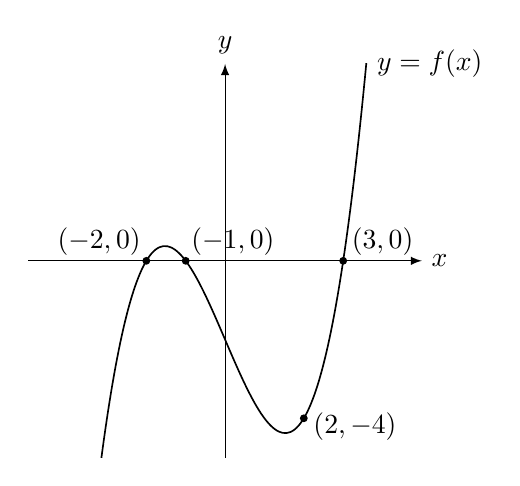
\begin{tikzpicture}[scale=.5]
      \tikzset{dot/.style={circle,fill,inner sep=1pt}}
      \tikzset{axis/.style={->,>=latex}}
      \begin{scope}
        \clip (-5,-5) rectangle (5,5);
        \draw[smooth,samples=100,domain=-5:5,semithick] plot (\x,{((\x*\x-7)*\x-6)/3});
      \end{scope}
      \draw[axis] (-5,0) -- (5,0) node[right] {$x$};
      \draw[axis] (0,-5) -- (0,5) node[above] {$y$};
      \node[dot] at (-2,0) {};
      \node at (-3.2,.5) {$(-2,0)$};
      \node[dot] at (-1,0) {};
      \node at (.2,.5) {$(-1,0)$};
      \node[dot] at (3,0) {};
      \node at (4,.5) {$(3,0)$};
      \node[dot] at (2,-4) {};
      \node at (3.3,-4.2) {$(2,-4)$};
      \node at (5.2,5) {$y=f(x)$};
    \end{tikzpicture}
  \end{center}
  \newpage
  \item 假設坐標平面的 $x$ 軸正向朝右,$y$ 軸正向朝上。已知 $A$、$B$ 兩動點目前分別位於 $(0,10)$ 與 $(0,-10)$,且 $A$、$B$ 兩點持續進行等速度運動,$A$ 點每秒向右移動 $3$ 單位,$B$ 點每秒向上移動 $4$ 單位。
  \begin{enumerate}[label=(\arabic*),left=0pt]
    \item 在 \blank{5em} 秒後兩動點間的距離會最短。
    \item 兩動點間的最短距離為 \blank{5em} 單位。
  \end{enumerate}
\end{enumerate}

\newpage
\label{hint}
{\bfseries\large 提示 \par}
\setcounter{section}{0}
\section{填充題}
\begin{enumerate}[label=\Alph*.,left=0pt]
  \item 
  \begin{enumerate}[label=(\arabic*),left=0pt]
    \item $y=ax^3 + bx^2 + cx + d$ 之圖形的對稱中心 $x$ 坐標會是 $-\fraction{b}{3a}$。
    \item 若 $f(x) = a(x-1)^3 + m(x-1)^2 + p(x-1) + k$,則 $f(x)$ 在 $x = 1$ 附近的一次近似為 $p(x - 1) + k$。
  \end{enumerate}
  \item 若有相異實數 $a$、$b$、$c$ 使 $f(a) = f(b) = f(c) = 0$,則由因式定理可知 $f(x)$ 會被 $(x-a)(x-b)(x-c)$ 整除。利用這個事實可以求出 $f(x)$。
  \item 設 $f(x)$ 為 $x$ 秒後兩動點間距離的平方,我們可以利用配方法求出 $f(x)$ 的最小值。
\end{enumerate}

\newpage
\label{answer}
{\bfseries\large 答案 \par}
\setcounter{section}{0}
\section{填充題}
\begin{enumerate}[label=\Alph*.,left=0pt]
  \item $(2,1)$;$2x-1$
  \item 10
  \item $\fraction{16}{5}$;$12$
\end{enumerate}
\end{document}
